\documentclass[10pt,a4paper]{article}

\usepackage[spanish]{babel}
\usepackage[utf8]{inputenc}
\usepackage{geometry}
\usepackage{url}
\usepackage{amsmath}
\usepackage{graphicx}
\usepackage{listings}
\usepackage{color}
\usepackage{multicol}
\definecolor{grey}{rgb}{0.8,0.8,0.8}
\usepackage{listings}
\usepackage{pdfpages}
\usepackage{csquotes}
\usepackage{float}
\usepackage{soul}
\usepackage{verbatim}
\usepackage{mips}
\usepackage{inconsolata}
% Configuración de lstlisting:

\lstset{
language=[mips]Assembler,
keywordstyle=\bfseries,
basicstyle=\ttfamily\small,
numberstyle=\footnotesize,
numbers=left,
stepnumber=2,
%backgroundcolor=\color{gray!10},
frame=single,
tabsize=4,
%rulecolor=\color{black!30},
title=\lstname,
escapeinside={\%*}{*)},
breaklines=true,
breakatwhitespace=true,
framextopmargin=2pt,
framexbottommargin=2pt,
extendedchars=true,
inputencoding=utf8,
literate={á}{{\'a}}1 {ó}{{\'a}}1 {é}{{\'e}}1,
}

\title{\textbf{Trabajo Práctico 1:\\ Conjunto de instrucciones MIPS}}

\author{Santiago Aguilera, \textit{Padrón Nro. 95795}\\
        \texttt{marquito.santi@gmail.com}\\
        Agustina Barbetta, \textit{Padrón Nro. 96528}\\
        \texttt{agustina.barbetta@gmail.com}\\
        Manuel Porto, \textit{Padrón Nro. 96587}\\
        \texttt{manu.porto94@hotmail.com}\\
        \\[2.5ex]
        \normalsize{2do. Cuatrimestre de 2016}\\
        \normalsize{66.20 Organización de Computadoras}\\
        \normalsize{Facultad de Ingeniería, Universidad de Buenos Aires}\\
       }


\begin{document}
\date{\today}

\maketitle

\thispagestyle{empty}
\begin{abstract}
El presente trabajo práctico consiste en crear parte de una aplicación, en MIPS32, capaz de dibujar los conjuntos fractales de Julia sobre una imagen de formato PGM.

El código del trabajo se encuentra en el siguiente repositorio: \\
\texttt{https://github.com/saantiaguilera/fiuba-orga-pc-julia-set}.\\
\end{abstract}

%\pagebreak

\tableofcontents

\pagebreak

\section{Descripción}
El objetivo del presente trabajo es familiarizarse con el conjunto de instrucciones MIPS y el concepto de ABI, extendiendo un programa que resuelva el problema descripto en secciones posteriores.

\section{Programa}
El trabajo consiste una modificacion de una seccion de un programa introducido en el TP0, que se encargaba de dibujar el conjunto de Julia y sus vecindades. La logica de computo del fractal debera tener soporte nativo para MIPS32 sobre NetBSD/pmax.

\subsection{Diseño}
A continuacion se describen los distintos componentes de la solucion.

\subsubsection{mips32\_plot}
La rutina \texttt{mips32\_plot} es una traducción del código C a la arquitectura MIPS32. La misma se encarga de el cálculo de color para cada píxel de la imagen y la escritura del archivo \texttt{.pgm}. 

Desde el punto de vista del usuario el programa funciona de manera idéntica al presentado en el primer trabajo. Sin embargo, para reducir la cantidad de \texttt{syscall}s utilizados se implemento un \textit{buffer} que almacena una determinada cantidad de elementos y solamente cuando el mismo se llena o termina la rutina, realiza la escritura del archivo. La razón de esta implementación es que las llamadas realizadas para escribir el archivo son costosas en tiempo, por lo que se busca reducirlas implementando un \textit{buffer} que escriba varios caracteres a la vez.

\subsubsection{write\_buffer}
Para implementar la lógica de la carga del \textit{buffer} y la escritura del archivo, se intentaron distintas soluciones. Una de ellas fue implementar la misma como una macro que se expandiría en su correspondiente código cada vez que fuera utilizada. Sin embargo, la versión de MIPS utilizada no soporta esta característica por lo que no fue posible implementar esta solución.

La solución alternativa consistió en dejar la lógica debajo de un \textit{label} y saltar a ella cada vez que se necesite.

\subsubsection{Stack Frame}
\begin{table}[H]
\centering
\begin{tabular}{c|c|}
\cline{2-2}
\textit{8260}  & \textit{a3}                \\ \cline{2-2}
\textit{8256}  & \textit{a2}                \\ \cline{2-2} 
\textit{8252}  & \textit{a1}                \\ \cline{2-2} 
\textit{8248}  & \textit{a0 (param)}                \\ \hline 
\textbf{8244}  & \textbf{fp}                \\ \cline{2-2} 
\textbf{8240}  & \textbf{gp}                \\ \cline{2-2} 
8236  & cpi                \\ \cline{2-2} 
8232  & cpr                \\ \cline{2-2}
8228  & c                \\ \cline{2-2} 
8224  & y                \\ \cline{2-2} 
8220  & x                \\ \cline{2-2} 
8216  & si                \\ \cline{2-2} 
8212  & sr                \\ \cline{2-2} 
8208  & zi                \\ \cline{2-2} 
8204  &  zr                \\ \cline{2-2} 
8200  &  ci                \\ \cline{2-2} 
8196  &  cr                \\ \cline{2-2}
8192  & buff\_len                \\ \cline{2-2}
8188  & buff (end)                 \\ 
8184  &                  \\ 
8180  &                  \\ 

  ... & ...             \\ 

8  &                  \\ 
4  &                  \\ 
0  & buff (start)                \\ \cline{2-2}
\end{tabular}
\caption{\textit{Stack frame} de la función \texttt{mips32\_plot()}. Las palabras 8248 a 8260 corresponden al \textit{Stack frame} de la función \texttt{caller}, las palabras en negrita corresponden a la \textit{General Register Save Area} y los restantes a la \textit{Local and Temporary Variables Area}.}
\end{table}

\begin{comment}
\subsubsection{Stack Frame}
\begin{table}[H]
\centering
\begin{tabular}{c|c|}
\cline{2-2}
\textit{2140}  & \textit{a3}                \\ \cline{2-2}
\textit{2136}  & \textit{a2}                \\ \cline{2-2} 
\textit{2132}  & \textit{a1}                \\ \cline{2-2} 
\textit{2128}  & \textit{a0 (params)}                \\ \hline 
\textbf{2124}  & \textbf{fp}                \\ \cline{2-2} 
\textbf{2120}  & \textbf{gp}                \\ \hline
2116  & data          \\ \cline{2-2}
2112  & data\_len               \\ \cline{2-2}
2108  & buffer\_addr                \\ \cline{2-2}
2104  & buffer\_len                \\ \cline{2-2}
2100  & ip (instruction pointer)                \\ \cline{2-2}
2096  & cpi                \\ \cline{2-2} 
2092  & cpr                \\ \cline{2-2} 
2088  & res                \\ \cline{2-2} 
2084  & c                \\ \cline{2-2} 
2080  & y                \\ \cline{2-2} 
2076  & x                \\ \cline{2-2} 
2072  & absz                \\ \cline{2-2} 
2068  & si                \\ \cline{2-2} 
2064  & sr                \\ \cline{2-2} 
2060  & zi                \\ \cline{2-2} 
2056  &  zr                \\ \cline{2-2} 
2052  &  ci                \\ \cline{2-2} 
2048  &  cr                \\ \cline{2-2}
2044  & buff (end)                 \\ \cline{2-2}
2040  &                  \\ \cline{2-2}
2036  &                  \\ \cline{2-2}

  ... & ...             \\ \cline{2-2}

8  &                  \\ \cline{2-2}
4  &                  \\ \cline{2-2}
0  & buff (start)                \\ \cline{2-2}
\end{tabular}
\caption{\textit{Stack frame} de la función \texttt{mips32\_plot()}. Las palabras 60 a 72 corresponden al \textit{Stack frame} de la función \texttt{caller}, las palabras en negrita corresponden a la \textit{General Register Save Area} y los restantes a la \textit{Local and Temporary Variables Area}.}
\end{table}

Para la variante con subrutina write:
\begin{table}[H]
\centering
\begin{tabular}{c|c|}
\cline{2-2}
\textit{84}  & \textit{a3}                \\ \cline{2-2}
\textit{80}  & \textit{a2}                \\ \cline{2-2} 
\textit{76}  & \textit{a1}                \\ \cline{2-2} 
\textit{72}  & \textit{a0 (params)}                \\ \hline 
\texttt{68}  & \texttt{padding}                \\ \cline{2-2}
\textbf{64}  & \textbf{ra}                \\ \cline{2-2} 
\textbf{60}  & \textbf{fp}                \\ \cline{2-2} 
\textbf{56}  & \textbf{gp}                \\ \cline{2-2}
\texttt{52}  & \texttt{padding}                \\ \cline{2-2}
48  & cpi                \\ \cline{2-2} 
44  & cpr                \\ \cline{2-2} 
40  & res                \\ \cline{2-2} 
36  & c                \\ \cline{2-2} 
32  & y                \\ \cline{2-2} 
28  & x                \\ \cline{2-2} 
24  & absz                \\ \cline{2-2} 
20  & si                \\ \cline{2-2} 
16  & sr                \\ \cline{2-2} 
12  & zi                \\ \cline{2-2} 
8  &  zr                \\ \cline{2-2} 
4  &  ci                \\ \cline{2-2} 
0  &  cr                \\ \cline{2-2} 
\end{tabular}
\caption{\textit{Stack frame} de la función \texttt{mips32\_plot()}. Las palabras 60 a 72 corresponden al \textit{Stack frame} de la función \texttt{caller}, las palabras en negrita corresponden a la \textit{General Register Save Area} y los restantes a la \textit{Local and Temporary Variables Area}.}
\end{table}

\begin{table}[H]
\centering
\begin{tabular}{c|c|}
\cline{2-2}
\textit{20}  & \textit{a3}                \\ \cline{2-2}
\textit{16}  & \textit{a2}                \\ \cline{2-2} 
\textit{12}  & \textit{a1}                \\ \cline{2-2} 
\textit{8}  & \textit{a0}                \\ \hline 
\textbf{4}  & \textbf{fp}                \\ \cline{2-2} 
\textbf{0}  & \textbf{gp}                \\ \cline{2-2}
\end{tabular}
\caption{\textit{Stack frame} de la función \texttt{write\_file}}
\end{table}


\begin{table}[H]
\centering
\begin{tabular}{c|c|}
\cline{2-2}
\textit{84}  & \textit{a3}                \\ \cline{2-2}
\textit{80}  & \textit{a2}                \\ \cline{2-2} 
\textit{76}  & \textit{a1}                \\ \cline{2-2} 
\textit{72}  & \textit{a0 (params)}                \\ \hline 
\textbf{68}  & \textbf{fp}                \\ \cline{2-2} 
\textbf{64}  & \textbf{gp}                \\ \cline{2-2}

60  & ip                \\ \cline{2-2} 
56  & len                \\ \cline{2-2} 
52  & data                \\ \cline{2-2}


48  & cpi                \\ \cline{2-2} 
44  & cpr                \\ \cline{2-2} 
40  & res                \\ \cline{2-2} 
36  & c                \\ \cline{2-2} 
32  & y                \\ \cline{2-2} 
28  & x                \\ \cline{2-2} 
24  & absz                \\ \cline{2-2} 
20  & si                \\ \cline{2-2} 
16  & sr                \\ \cline{2-2} 
12  & zi                \\ \cline{2-2} 
8  &  zr                \\ \cline{2-2} 
4  &  ci                \\ \cline{2-2} 
0  &  cr                \\ \cline{2-2} 
\end{tabular}
\caption{\textit{Stack frame} de la función \texttt{mips32\_plot()}. Las palabras 60 a 72 corresponden al \textit{Stack frame} de la función \texttt{caller}, las palabras en negrita corresponden a la \textit{General Register Save Area} y los restantes a la \textit{Local and Temporary Variables Area}.}
\end{table}
\end{comment}

\subsection{Compilación}
El código fuente provisto por la cátedra provee los makefiles necesarios para compilar el
ejecutable a partir de la versión en C con el archivo \texttt{mips32\_plot.c}. Para poder compilar el
código desarrollado se debió cambiar la definición en el archivo Makefile 6:

\texttt{SRCS = mips32\_plot.c main.c mygetopt\_long.c}

por

\texttt{SRCS = mips32\_plot.S main.c mygetopt\_long.c}

Luego deberán invocar la siguiente secuencia de comandos para limpiar los archivos temporales
y generar los nuevos Makefiles:
\begin{lstlisting}[  frame=top,frame=bottom,
  basicstyle=\footnotesize\normalfont\ttfamily,%\sffamily,    % the size of the fonts that are used for the code
  stepnumber=0,                           % the step between two line-numbers. If it is 1 each line will be numbered
  numbersep=10pt,                         % how far the line-numbers are from the code
  tabsize=2,                              % tab size in blank spaces
  extendedchars=true,                     %
  breaklines=true,                        % sets automatic line breaking
  captionpos=t,                           % sets the caption-position to top
  mathescape=true,
  stringstyle=\color{white}\ttfamily, % Farbe der String
  showspaces=false,           % Leerzeichen anzeigen ?
  showtabs=false,             % Tabs anzeigen ?
  xleftmargin=17pt,
  framexleftmargin=17pt,
  framexrightmargin=17pt,
  framexbottommargin=5pt,
  framextopmargin=5pt,
  showstringspaces=false      % Leerzeichen in Strings anzeigen ?
  ]
> make clean
> make makefiles
> make

\end{lstlisting}

Para la compilación del programa se cuenta con un \textit{Makefile}, el mismo cuenta con un\textit{ phony target} para limpiar los archivos generados (\texttt{make clean}) y el target \textit{phony all} que (por más que sea \textit{phony}) generará un ejecutable '\texttt{tp0}' y los archivos del \textit{linker} necesarios (\texttt{make} o \texttt{make all}).

\subsection{Pruebas}

Se creó una \textit{test-suite} en bash para testear casos borde de los parámetros y que el programa funcione correctamente. 

Para correrla simplemente hay que compilar el proyecto previamente, darle permisos al \textit{script} (de ser necesarios, \texttt{chmod u+x run\_tests.sh}) y correrlo de forma normal (\texttt{bash run\_tests.sh}). El mismo irá dando información sobre cada test corrido y su estado.

Las mismas se encargan de probar el pasaje de argumentos en casos particulares (pasar caracteres en vez de numeros, poner datos no respetando el formato, entre otros) y a su vez de correr el caso de exito. Actualmente, el programa cuenta con una limitacion, la cual es que, si se cambia el size del buffer a "1" (o un numero menor al size de un color, el cual puede ir entre 1 y 3 bytes), el buffer nunca podra llenarse y por consiguiente no se escribira nada. Por lo cual se tiene como pre condicion que el size del buffer sea siempre mayor o igual a 4 (porque consideramos tambien el salto de linea)

\section{Conclusiones}
La realización de este trabajo fue importante para entender y aplicar los temas vistos en clase sobre MIPS y su ABI. A su vez, se pudo ver detalladamente el funcionamiento de un programa assembly, y particularmente el funcionamiento del stack en el mismo. 

\section{Apéndices}

\subsection{Código fuente}
El código a continuación se encuentra también en el repositorio del trabajo: \\
\texttt{https://github.com/saantiaguilera/fiuba-orga-pc-julia-set}.\\

\lstinputlisting[caption=mips32\_plot.S]{mips32_plot.S}

\subsection{Enunciado}
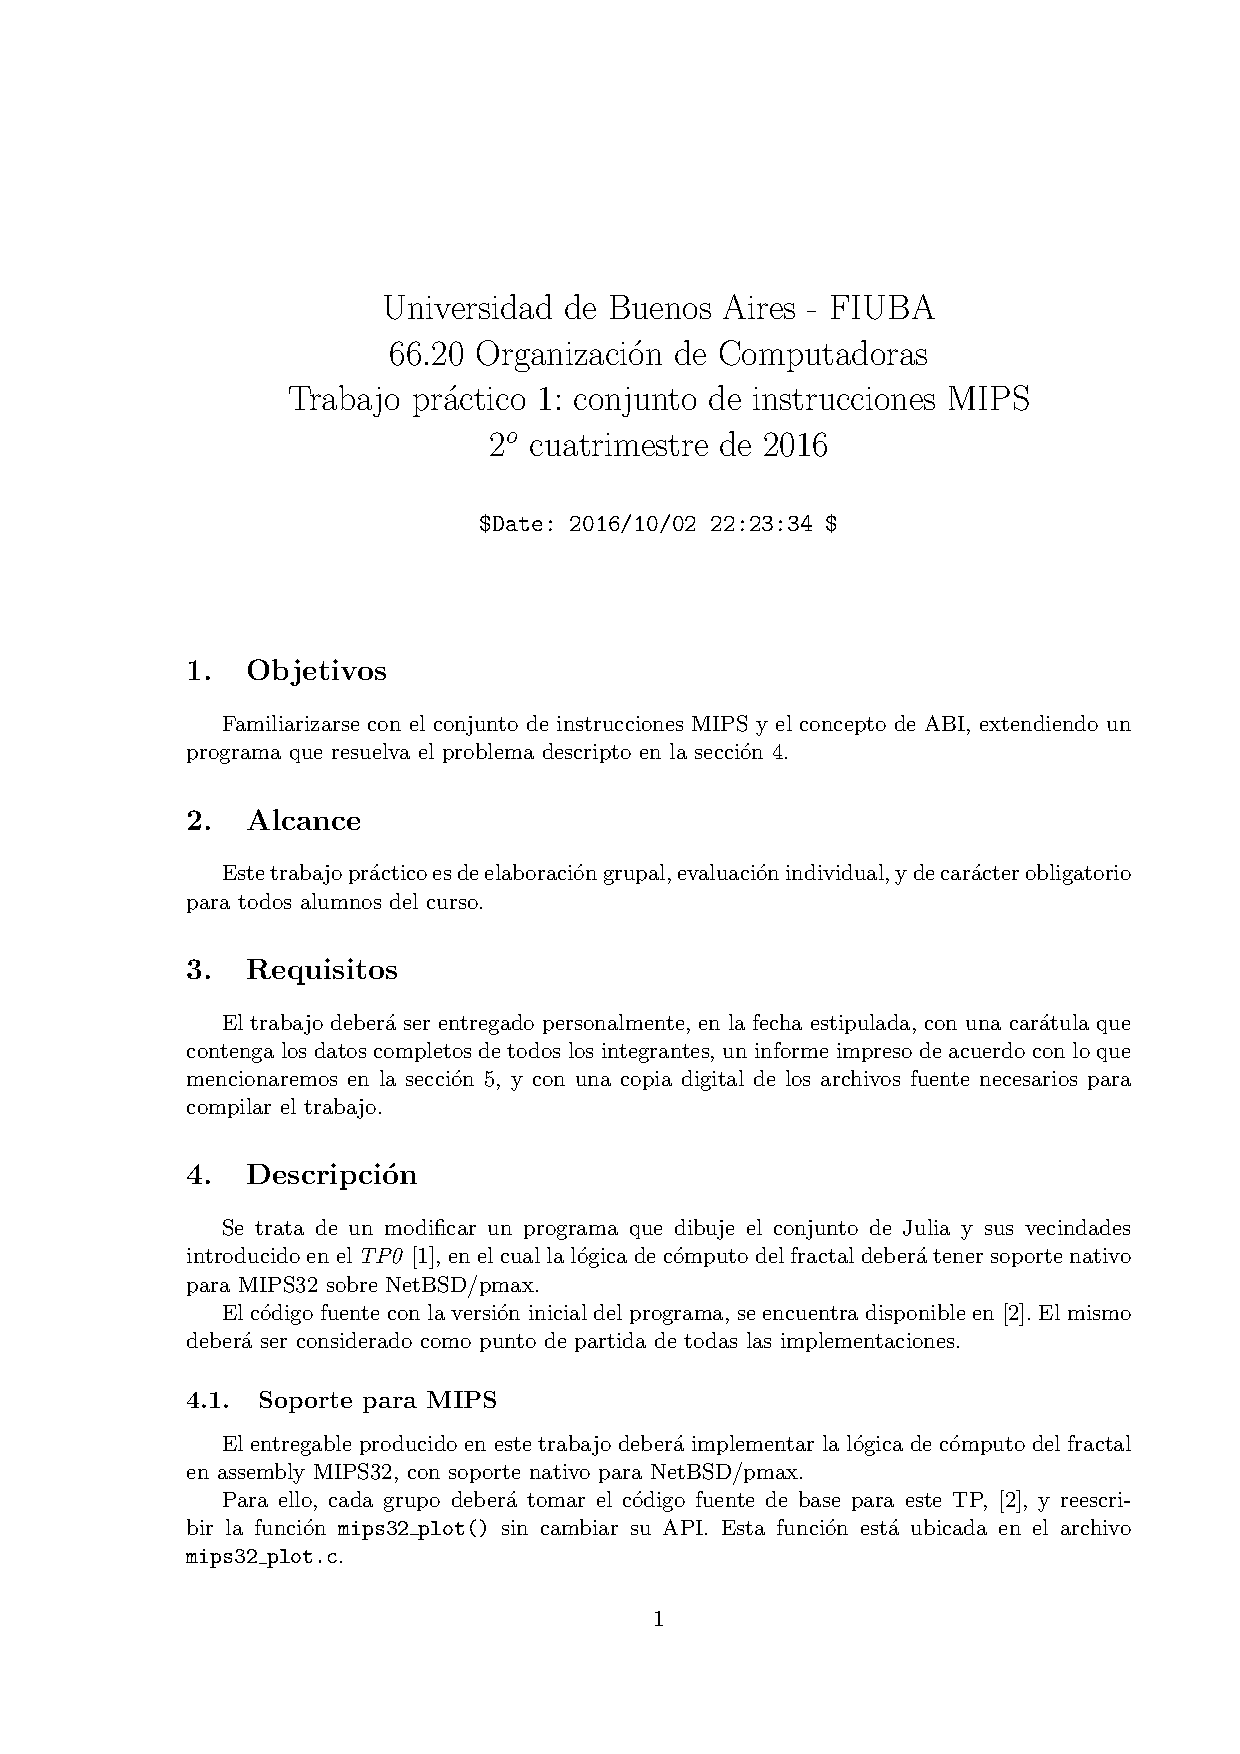
\includepdf[pages={-}]{enunciado.pdf}



\begin{thebibliography}{99}
\bibitem{Gxemul} \emph{GXemul}\\
\url{http://gavare.se/gxemul/}

\bibitem{NetBSD} \emph{The NetBSD project}\\
\url{http://www.netbsd.org/}

\bibitem{Juli} \emph{Conjunto de Julia}\\
\url{https://es.wikipedia.org/wiki/Conjunto_de_Julia}

\end{thebibliography}
\end{document}
